
\chapter{Version Control}
\label{cha:version-control}



A version control system gives you automated help at keeping a change history for a file or group of files.
It allows you to recover any stage in that history, and it makes getting reports on the differences between versions easy.


Here we use Git as the version control system.
In Emacs, we use Magit.
Magit is an interface to the version control system Git, implemented as an Emacs package.


\section{Installation}
\label{sec:installation-1}
In you \argument{.emacs} or \argument{.emacs.el} file, add the following code.

\begin{lstlisting}
;; Use package manager interface.
(require 'package)

;; Add melpa site to package archives.
;; This is used define where to fetch package. 
(add-to-list 'package-archives '("melpa-stable" . "https://stable.melpa.org/packages/") t)

;; Load Emacs Lisp packages, and activate them.
(package-initialize)


;; Install Magit
(package-install 'magit)
\end{lstlisting}

\section{Basic}
\label{sec:basic}

\subsection{Show Status Buffer}
\label{sec:show-status-buffer}


Type \keyword{C-x g} to display information about the current Git repository in a dedicated buffer, called the status buffer. If the current directory isn’t located within a Git repository, then prompt for an existing repository or an arbitrary directory, depending on option ``magit-repository-directories'', and show the status of the selected repository instead.

\begin{itemize}
\item If that option specifies any existing repositories, then offer those for completion and show the status buffer for the selected one.
\item Otherwise read an arbitrary directory using regular file-name completion.  If the selected directory is the top-level of an existing working tree, then show the status buffer for that.
\item Otherwise offer to initialize the selected directory as a new repository.  After creating the repository show its status buffer.
\end{itemize}

Depending on what state your repository is in, this buffer may contain sections titled ``Staged changes'', ``Unstaged changes'', ``Unmerged into origin/master'', ``Unpushed to origin/master'', and many others.

Move between sections using \keyword{p} and \keyword{n}.
Note that the bodies of some sections are hidden.
Type \keyword{TAB} to expand or collapse the section at point.
You can also use \keyword{C-tab} to cycle the visibility of the current section and its children. 

\begin{tcolorbox}
  In status buffer, remember use \keyword{C-h m} to get help information about this mode.
\end{tcolorbox}


\subsection{Stage and Unstage}
\label{sec:stage-unstage}

Move to a file section inside the section named ``Unstaged changes'' and type \keyword{s} to stage the changes you have made to that file.
That file now appears under ``Staged changes''.

Magit can stage and unstage individual hunks, not just complete files.
Move to the file you have just staged, expand it using \keyword{TAB}, move to one of the hunks using \keyword{n}, and unstage just that by typing \keyword{u}.
Note how the staging (\keyword{s}) and unstaging (\keyword{u}) commands operate on the change at point.
Many other commands behave the same way.


You can also un-/stage just part of a hunk.
Inside the body of a hunk section (move there using \keyword{C-n}), set the mark using \keyword{C-SPC} and move down until some added and/or removed lines fall inside the region but not all of them.
Again type \keyword{s} to stage.

It is also possible to un-/stage multiple files at once.
Move to a file section, type \keyword{C-SPC}, move to the next file using \keyword{n}, and then \keyword{s} to stage both files.

\subsection{Commit}
\label{sec:commit}

If you want to commit your changes.
Type \keyword{c}.
This shows the available commit commands and arguments in a buffer at the bottom of the frame.
Each command and argument is prefixed with the key that invokes/sets it.
If you want to create a ``normal'' commit, just type \keyword{c} again.


Now two new buffers appear.
One is for writing the commit message, the other shows a diff with the changes that you are about to commit.
Write a message and then type \keyword{C-c C-c} to actually create the commit.

\subsection{Push}
\label{sec:push}

You can push it by typing \keyword{p} to show all the available push commands and arguments and then \keyword{p} to push to a branch with the same name as the local branch onto the remote configured as the push-remote.
If the push-remote is not configured yet, then you would first be prompted for the remote to push to.


\subsection{Transient prefix commands}
\label{sec:help}

To show a menu that lists all menus, type \keyword{h}.
(Such menus are also called ``transient prefix commands'' or just ``transients''.)

\keyword{C-x M-g} is the global binding of this menu.
You can invoke this menu even not in status buffer.
In file visiting buffers \keyword{C-c M-g} brings up a similar menu featuring commands that act on just the visited file.

\begin{figure}[!htbp]
  \centering
  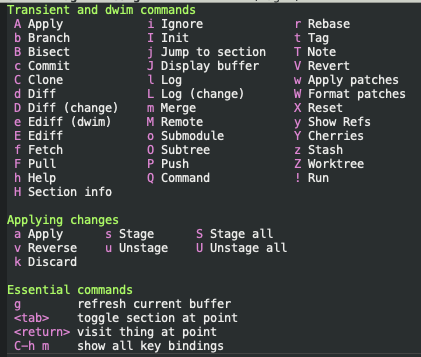
\includegraphics[width=\textwidth]{transient-commands}
  \caption{Transient prefix commands}
  \label{fig:transient-commands}
\end{figure}

\newpage{}
\subsection{Summary}
\label{sec:summary}

\begin{table}[H]
  \centering
  \begin{tabular}{>{\bfseries}lp{0.6\textwidth}}
    \toprule
    \head{Binding} & \head{Meaning} \\
    \midrule
    C-x g & Show the status of the current Git repository in a buffer.\\
    TAB & expand or hide the section at point.\\
    C-TAB & Cycle the visibility of the current section and its children.\\
    RET & visit the change or commit at point\\
    n & Move to the beginning of the next visible section.\\
    p & Move to the beginning of the current or the previous visible section.\\
    s & stage\\
    u & unstage\\
    c & commit\\
    p & push\\
    h & invoke major commands\\
    C-x M-g & invoke major commands\\
    C-c M-g & invoke major commands that act on just the visited file\\
    \bottomrule
  \end{tabular}
  \caption{Basic magit commands}
  \label{tab:basic-magit-commands}
\end{table}





% Here are some commands used in status buffer shown in Table \ref{tab:magit-cmds}.
% \begin{center}
%   \begin{longtable}[H]{>{\bfseries}lp{0.6\textwidth{}}}
      %       \toprule
      %       \head{Binding} & \head{Meaning}\\
      %       \midrule
      %       \endfirsthead

      %       \toprule
      %       \head{Binding} & \head{Meaning}\\
      %       \midrule
      %       \endhead

      %       \midrule
      %       \multicolumn{2}{c}{{Continued on next page}}\\
      %       \bottomrule
      %       \endfoot

      %       \endlastfoot

      %       \midrule
      %       SPC & Either show the commit or stash at point in the appropriate buffer, or if that buffer is already being displayed in the current frame and contains information about that commit or stash, then instead scroll the buffer up.  If there is no commit or stash at point, then prompt for a commit.\\
      %       ! & Run git or another command, or launch a graphical utility.\\
      %       \$ & Display the current repository’s process buffer.\\
      %       \% & Act on a worktree.\\
      %       + & Increase the context for diff hunks by COUNT(\keyword{C-u n}) lines.\\
      %       - & Decrease the context for diff hunks by COUNT(\keyword{C-u n}) lines.\\
      %       0 & Reset context for diff hunks to the default height.\\
      %       1 & Show surrounding sections on first level.\\
      %       2 & Show surrounding sections up to second level.\\
      %       3 & Show surrounding sections up to third level.\\
      %       4 & Show surrounding sections up to fourth level.\\
      %       : & Execute COMMAND asynchronously; display output.\\
      %       < & Move point to the beginning of the buffer.\\
      %       > & Move point to the end of the buffer.\\
      %       \bottomrule
      %       \caption{Magit commands\label{tab:magit-cmds}}
      %     \end{longtable}
      %       \end{center}

\section{Interface Concepts}
\label{sec:interface-concepts}

\subsection{Modes and Buffers}
\label{sec:modes-buffers}


Magit provides several major-modes.
For each of these modes there usually exists only one buffer per repository.
Separate modes and thus buffers exist for commits, diffs, logs, and some other things.

Besides these special purpose buffers, there also exists an overview buffer, called the status buffer.
It’s usually from this buffer that the user invokes Git commands, or creates or visits other buffers.


\begin{table}[H]
  \centering
  \begin{tabular}{>{\bfseries}lp{0.6\textwidth}}
    \toprule
    \head{Binding} & \head{Meaning}\\
    \midrule
    q & Bury the current buffer. With a prefix argument, kill the buffer instead. With two prefix arguments, also kill all Magit buffers associated with this repository.\\
    g & Refresh the current buffer if its major mode derives from ``magit-mode'', and refresh the corresponding status buffer.\\
    G & Refreshes all Magit buffers belonging to the current repository and also reverts all unmodified buffers that visit files being tracked in the current repository.\\
    \bottomrule
  \end{tabular}
  \caption{Modes and buffers commands}
  \label{tab:modes-buffers-cmds}
\end{table}

\subsection{Sections}
\label{sec:sections}

Magit buffers are organized into nested sections, which can be collapsed and expanded, similar to how sections are handled in Org mode.
Each section also has a type, and some sections also have a value.
For each section type there can also be a local keymap, shared by all sections of that type.

Taking advantage of the section value and type, many commands operate on the current section, or when the region is active and selects sections of the same type, all of the selected sections.
Commands that only make sense for a particular section type are usually bound in section type keymaps.

\begin{table}[H]
  \centering
  \begin{tabular}{>{\bfseries}lp{0.6\textwidth}}
    \toprule
    \head{Binding} & \head{Meaning}\\
    \midrule
    n & Move to the beginning of the next visible section.\\
    p & Move to the beginning of the current or the previous visible section.\\
    M-p & Move to the beginning of the previous sibling section. If there is no previous sibling section, then move to the parent section instead.\\
    M-n & Move to the beginning of the next sibling section. If there is no next sibling section, then move to the parent section instead.\\
    \textasciicircum{} & Move to the beginning of the parent of the current section.\\
    \midrule
    TAB & Expand or hide the section at point.\\
    C-TAB & Cycle the visibility of current section and its children.\\
    magit-section-cycle-diffs & Cycle the visibility of diff-related sections in the current buffer.\\
    magit-section-cycle-global & Cycle the visibility of all sections in the current buffer.\\
    \midrule
    1 & \multirow{4}{*}{Show sections surrounding the current section up to level N.}\\
    2 & \\
    3 & \\
    4 & \\
    \midrule
    M-1 & \multirow{4}{*}{Show all sections up to level N.}\\
    M-2 & \\
    M-3 & \\
    M-4 & \\
    \midrule
    H & Shows information about the section at point in a separate buffer.\\
    \bottomrule
  \end{tabular}
  \caption{Sections commands}
  \label{tab:sections-cmds}
\end{table}

\subsection{Transient Commands}
\label{sec:transient-commands}

Many Magit commands are implemented as transient commands.
First the user invokes a prefix command, which causes its infix arguments and suffix commands to be displayed in the echo area.
The user then optionally sets some infix arguments and finally invokes one of the suffix commands.


\subsection{Transient Arguments and Buffer Variables}
\label{sec:trans-argum-buff}

The infix arguments of many of Magit’s transient prefix commands cease to have an effect once the git command that is called with those arguments has returned.
Commands that create a commit are a good example for this.
If the user changes the arguments, then that only affects the next invocation of a suffix command.
If the same transient prefix command is later invoked again, then the arguments are initially reset to the default value.
It is possible to cycle through previously used sets of arguments using \keyword{C-M-p} and \keyword{C-M-n}.

\begin{figure}[!htbp]
  \centering
  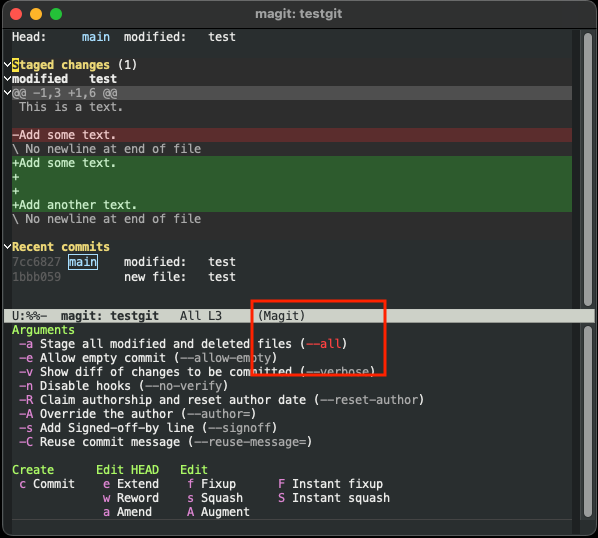
\includegraphics[width=0.7\textwidth]{transient-commit-1}
  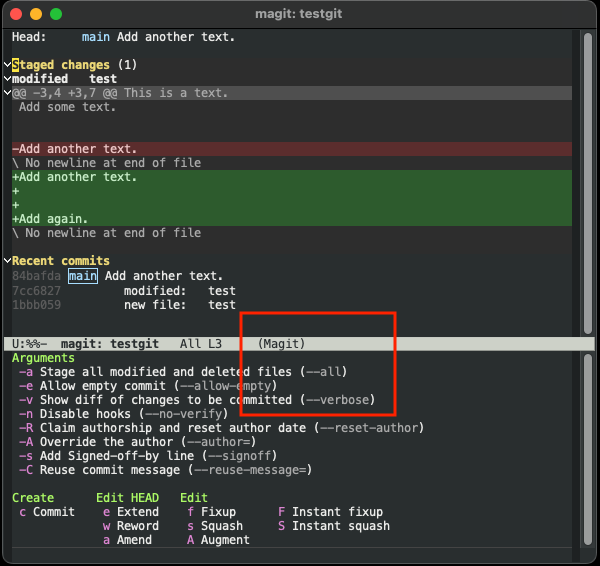
\includegraphics[width=0.7\textwidth]{transient-commit-2}
  \caption{Transient commit arguments}
  \label{fig:transient-commit-arguments}
\end{figure}


Figure \ref{fig:transient-commit-arguments} show this effect.
After the commit, the next time you commit, the argument is reset to the default value.


However the infix arguments of many other transient commands continue to have an effect even after the git command that was called with those arguments has returned.
The most important commands like this are those that display a diff or log in a dedicated buffer.
Their arguments obviously continue to have an effect for as long as the respective diff or log is being displayed.
Furthermore the used arguments are stored in buffer-local variables for future reference.
We can also use \keyword{C-M-p} and \keyword{C-M-n} to previous and next arguments stored in buffer-local variables.


It is also possible to change the diff and log arguments used in the current buffer (including the status buffer, which contains both diff and log sections) using the respective ``refresh'' transient prefix commands on \keyword{D} and \keyword{L}.
(\keyword{d} and \keyword{l} on the other hand are intended to change what diff or log is being displayed.
It is possible to also change how the diff or log is being displayed at the same time, but if you only want to do the latter, then you should use the refresh variants.)
Because these secondary diff and log transient prefixes are about changing the arguments used in the current buffer, they always start out with the set of arguments that are currently in effect in that buffer.

\begin{figure}[!htbp]
  \centering
  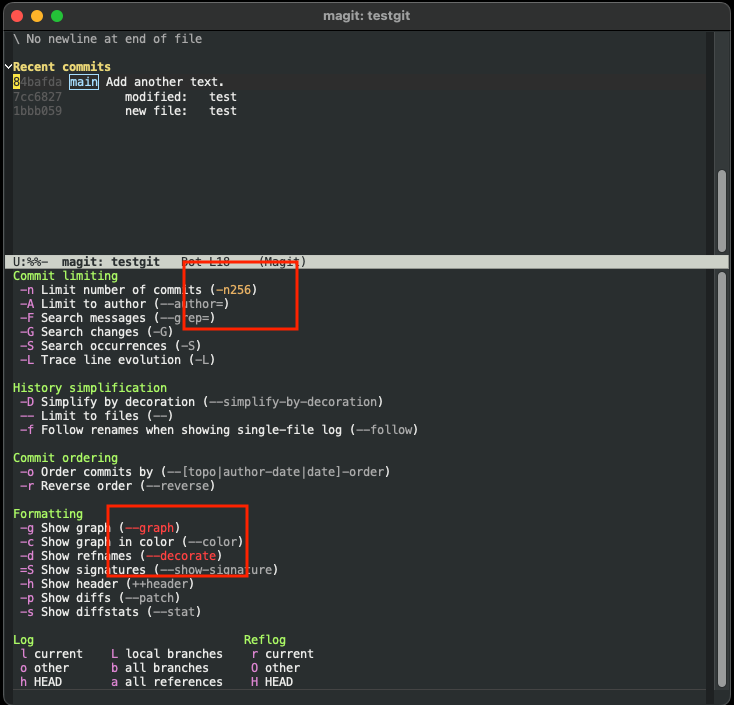
\includegraphics[width=0.8\textwidth]{transient-log}
  \caption{Transient log arguments}
  \label{fig:transient-log-arguments}
\end{figure}

Figure \ref{fig:transient-log-arguments} show this effect.
The arguments are still there.

\subsection{Running Git}
\label{sec:running-git}

Magit runs Git either for side-effects (e.g. when pushing) or to get some value (e.g. the name of the current branch).
When Git is run for side-effects, the process output is logged in a per-repository log buffer, which can be consulted using the \keyword{magit-process} command when things don't go as expected.



\begin{table}[H]
  \centering
  \begin{tabular}{>{\bfseries}lp{0.6\textwidth}}
    \toprule
    \head{Binding} & \head{Meaning}\\
    \midrule
    \$ & Displays the process buffer for the current repository.\\
    k & Kills the process represented by the section at point.\\
    ! & Run git command\\
    \bottomrule
  \end{tabular}
  \caption{Git commands}
  \label{tab:Git-cmds}
\end{table}

\section{Inspecting}
\label{sec:inspecting}

The functionality provided by Magit can be roughly divided into three groups:
\begin{itemize}
\item inspecting existing data
\item manipulating existing data or adding new data
\item transferring data
\end{itemize}


\begin{table}[H]
  \centering
  \begin{tabular}{l>{\bfseries}lp{0.6\textwidth}}
    \toprule
    \head{Group} & \head{Binding} & \head{Meaning}\\
    \midrule
    status & C-x g & Show status buffer.\\
    \midrule
    \multirow{3}{*}{logging} & l & show a commit or reference log.\\
                 & L & Change the arguments used for the log(s) in the current buffer.\\
                 & Y & Show commits that are in a certain branch but that have not been merged in the upstream branch.\\
    \midrule
    \multirow{2}{*}{diffing} & d & Show changes between different versions.\\
                 & D & Change the arguments used for the diff(s) in the current buffer.\\
    \midrule
    \multirow{2}{*}{ediffing} & e & Compare, stage, or resolve using Ediff. This command tries to guess what file, and what commit or range the user wants to compare, stage, or resolve using Ediff.\\
                 & E & Show differences using the Ediff package.\\
    \midrule
    references & y & Lists branches and tags in a dedicated buffer.\\
    \midrule
    bisecting & B & Narrow in on the commit that introduced a bug.\\
    \bottomrule
  \end{tabular}
  \caption{Inspecting Commands}
  \label{tab:inspecting-commands}
\end{table}


\newpage{}

\section{Manipulating}
\label{sec:manipulating}


\begin{table}[H]
  \centering
  \begin{tabular}{l>{\bfseries}lp{0.6\textwidth}}
    \toprule
    \head{Group} & \head{Binding} & \head{Meaning}\\      
    \midrule
    init & I & Initialize a repository and then shows the status buffer for the new repository.\\
    \midrule
    clone & C & Clone a repository.\\
    \midrule
    \multirow{2}{*}{staging} & s & Add the change at point to the staging area.\\
                 & S & Stage all changes to files modified in the worktree.\\
    \midrule
    \multirow{2}{*}{unstaging} & u & Remove the change at point from the staging area.\\
                 & U & Remove all changes from the staging area.\\
    \midrule
    \multirow{3}{*}{applying} & a & Apply the change at point to the working tree.\\
    & k & Remove the change at point from the working tree.\\
    & v & Reverse the change at point in the working tree.\\
    \midrule
    commit & c & Reverse the change at point in the working tree.\\
    \midrule
    branching & b & Add, configure or remove a branch.\\
    \midrule
    merging & m & Merge branches.\\
    \midrule
    rebasing & r & Transplant commits and/or modify existing commits.\\
    \midrule
    \multirow{2}{*}{cherry picking} & A & Apply or transplant commits.\\
                 & V & Revert existing commits, with or without creating new commits.\\
    \midrule
    resetting & x & Reset the HEAD and index to some commit read from the user and defaulting to the commit at point, and possibly also reset the working tree. With a prefix argument reset the working tree otherwise don't.\\
                 & X & Reset the HEAD and index to some commit read from the user and defaulting to the commit at point. The working tree is kept as-is.\\
    \midrule
    stashing & z & Stash uncommitted changes.\\
    \midrule
    \midrule
    tag & t & Create or delete a tag.\\
    \midrule
    note & T & Edit notes attached to commits.\\
    \midrule
    submodules & o & Act on a submodule.\\
    \midrule
    subtree & O & Import or export subtrees.\\
    \midrule
    worktree & Z & Act on a worktree.\\
    \bottomrule
  \end{tabular}
  \caption{Manipulating commands}
  \label{tab:manipulating-cmds}
\end{table}


\section{Transferring}
\label{sec:transferring}

\begin{table}[H]
  \centering
  \begin{tabular}{l>{\bfseries}lp{0.6\textwidth}}
    \toprule
    \head{Group} & \head{Binding} & \head{Meaning}\\      
    \midrule
    remote & M & Add, configure or remove a remote.\\
    \midrule
    fetching & f & Fetch from repository.\\
    \midrule
    pulling & F & Pull from repository.\\
    \midrule
    pushing & P & Push to repository.\\
    \midrule
    \multirow{2}{*}{patches} & W & Create or apply patches.\\
                 & w & Apply patches received by email.\\
    \bottomrule
  \end{tabular}
  \caption{Manipulating commands}
  \label{tab:manipulating-cmds}
\end{table}


%%% Local Variables:
%%% mode: latex
%%% TeX-master: "emacs"
%%% End:
